%%%%%%%%%%%%%%%%%%%%%%%%%%%%%%%%%%%%%%%%%%%%%%%%%%%%%%%%%%%%%%%%%%%%%%%%
% Golden Sacra - Memoria
% Escuela Politécnica Superior de la Universidad de Alicante
% Realizado por: Ángel Jesús Terol Martínez
% Contacto: jtm37@alu.ua.es
%%%%%%%%%%%%%%%%%%%%%%%%%%%%%%%%%%%%%%%%%%%%%%%%%%%%%%%%%%%%%%%%%%%%%%%%
\chapter{Anexo}
\label{anexo}

\section{CPU}

Como ya has podido comprobar, la CPU que la Game Boy utiliza es la \textbf{Sharp LR35902}, variante de la \textbf{Zilog Z80} e \textbf{Intel 8080}. Es un procesador de \textbf{8 bits} que puede realizar \textbf{cálculos de 16 bits} y \textbf{manejar hasta 64Kb de memoria externa} para el control del Joypad, el LCD o el control de sonido. A pesar de ello, se queda lejos de poseer todas las características de la Zilog Z80. Las operaciones de 16 bits que posee son muy reducidas, pues no posee instrucciones con prefijos \textbf{ED}, \textbf{FD} ni \textbf{DD}\footnote{Denominados ``Undocumented opcodes'', los cuales no están en la lista oficial del Zilog.}. Esto implica que \textbf{no disponemos} tampoco de los registros \textbf{IX}.

\subsection{Registros}

Para poder empezar a programar en ensamblador \textbf{debemos saber qué registros tenemos y cómo usar cada uno de ellos}. Los nombres de los registros de los que disponemos son A, F, B, C, D, E, H, y L, los cuales pueden contener \textbf{1 byte} de información. También \textbf{pueden ser agrupados} en pares de forma que puedan contener \textbf{2 bytes}: AF, BC, DE y HL. También están los registros SP y PC, los cuales tienen una \textbf{función específica} dentro de la CPU.
\\ \\
En primer lugar tenemos el registro \textbf{A}, también denominado \textbf{Acumulador}. Es donde va a estar la mayor parte de la información procesada. Es un registro al que se le puede \textbf{introducir valores de forma directa}, al igual que B, C, D, E, H y L.
\\ \\
Los registros \textbf{B} y \textbf{C} se suelen usar para \textbf{contadores} y los registros \textbf{D} y \textbf{E} como un par de 2 bytes para almacenar \textbf{direcciones de memoria} sobre las que copiar distintos datos. Obviamente, sus usos no están limitados a las dos que acabo de mencionar, depende de lo que el programador vea conveniente en cada momento.
\\ \\
El registro \textbf{F} (o \textbf{Flags}) es donde se almacena en todo momento el \textbf{estado del procesador}. Es un registro de \textbf{solo lectura}, aunque puede utilizarse junto a A para distintas operaciones. Se suele usar a la hora de \textbf{comprobar el resultado de la instrucción anterior}. En la siguiente tabla puedes ver la función de cada uno de los bits:

\begin{table}[h!]
\centering
\begin{tabular}{|l|l|l|l|l|}

\hline

\multicolumn{5}{|c|}{\textbf{Flags}}                                                                                                                 \\ \hline

\multicolumn{1}{|c|}{\textbf{Bit}} & \multicolumn{1}{c|}{\textbf{Nombre}} & \multicolumn{1}{c|}{\textbf{0}} & \multicolumn{1}{c|}{\textbf{1}} & \multicolumn{1}{c|}{\textbf{Definición}} \\ \hline

7                         & zf                          & Z                      & NZ                     & Flag Zero                       \\ \hline

6                         & n                           & -                      & -                      & Flag de suma/resta              \\ \hline

5                         & h                           & -                      & -                      & Flag de semi acarreo            \\ \hline

4                         & cy                          & C                      & NC                     & Flag de acarreo                 \\ \hline

3-0                       & -                           & -                      & -                      & Sin uso.                        \\ \hline
\end{tabular}

\caption{Función de los bits del registro F o Flags}

\label{table:2}
\end{table}

Los registros \textbf{H} y \textbf{L} se utilizan para \textbf{acceso indirecto a una dirección de memoria}. Con acceso indirecto nos referimos al valor de 16 bits que contiene la dirección HL. Es muy útil a la hora de recorrer los valores de un determinado array.
\\ \\
Los registros \textbf{SP} (\textbf{Stack Pointer}) se utilizan para \textbf{conocer la posición de memoria desde la cual se hizo una llamada}. Es decir, cuando hacemos una instrucción ``call'', la pila aumenta, y al hacer un ``ret'', disminuye de tamaño.
\\ \\
Y por último, los registros \textbf{PC} (\textbf{Program Counter}), los cuales indican la dirección de memoria de la \textbf{próxima instrucción} que se va a ejecutar.

\subsection{Instrucciones}

No voy a entrar en detalle a cerca de las instrucciones que existen, porque para estos casos lo mejor es visitar cualquier tabla con todos los opcodes\footnote{También conocido como \textbf{Operation Code}. Es una porción de código máquina que especifica la instrucción a realizar.} que tiene la CPU (en la bibliografía hay un enlace a una de ellas que me ha resultado muy útil).
\\ \\ 
A grosso modo, las instrucciones las podemos calificar de la siguiente manera:

\begin{itemize}
	\item \textbf{Operaciones de carga:} LD, PUSH, POP...
    \item \textbf{Manipulación de bits:} BIT, SET y RES.
    \item \textbf{Operaciones aritméticas de 8 bits:} AND, OR, XOR, ADD...
    \item \textbf{Operaciones aritméticas de 16 bits:} RRA, RLA, RRC, SLA...
    \item \textbf{Operaciones de salto:} JP, JR, RET, RETI y CALL.
    \item \textbf{Definiciones de espacio:} DB, DS, DW...
    \item \textbf{Operaciones de uso general:} HALT, DI, EI, STOP...
\end{itemize}

Para una \textbf{información más detallada} de lo que hace cada operación lo mejor es consultar el \textbf{manual oficial de la CPU} o similares. En la bibliografía podrás encontrarlos.

\clearpage

\section{Mapa de memoria}
\label{memory_map}

Como hemos comentado con anterioridad, la Game Boy nos permite direccionar directamente un total de \textbf{64Kb de memoria} (esto es, en hexadecimal, desde la posición \$0000 hasta la \$FFFF). Esta memoria está \textbf{dividida en distintos bloques}, mapeados por los diseñadores de aquel entonces, dejando a la \textbf{ROM con dos bloques de 16Kb}, y \textbf{un bloque de 8Kb} para la \textbf{RAM}. Aún así, estos espacios de memoria eran insuficientes para algunos videojuegos, con lo que se pasó a emplear la técnica del \textbf{\textit{Banking}}. Esta técnica consistía en dividir una vez más la ROM en distintos bloques, cada uno independiente del otro, de forma que siempre tendríamos un \textbf{bloque fijo} de 16Kb donde almacenaríamos toda la \textbf{lógica del juego} y, mediante ciertas instrucciones, \textbf{cambiar el segundo bloque} de 16Kb por otro de igual tamaño según las necesidades del programador.

En la siguiente tabla podemos ver los distintos bloques ya mencionados:

\begin{table}[h!]
\centering
\begin{tabular}{ |c|c|c| }
\hline
\multicolumn{3}{|c|}{\textbf{Mapa de memoria}}              \\ \hline
\textbf{Inicio} & \textbf{Final} & \textbf{Descripción}     \\ \hline
0000   & 3FFF  & Banco 00, 16Kb ROM                         \\ \hline
4000   & 7FFF  & Banco 01 - NN, 16Kb ROM                    \\ \hline
8000   & 9FFF  & 8Kb Video RAM                              \\ \hline
A000   & BFFF  & 8Kb RAM externa                            \\ \hline
C000   & CFFF  & Banco 00, 4Kb RAM interna                  \\ \hline
D000   & DFFF  & Banco 01 - NN, 4Kb RAM interna             \\ \hline
E000   & FDFF  & Espejo de la RAM interna                   \\ \hline
FE00   & FE9F  & OAM                                        \\ \hline
FEA0   & FEFF  & No usable                                  \\ \hline
FF00   & FF7F  & Registros Entrada/Salida                   \\ \hline
FF80   & FFFE  & High RAM                                   \\ \hline
FFFF   & FFFF  & Registro de activación de interrupciones   \\ \hline
\end{tabular}
\caption{Mapa de Memoria de la Game Boy}
\label{table:3}
\end{table}

Como podemos ver, los dos primeros bloques (\textbf{\$0000 - \$7FFF}) se utilizan para acceder a la ROM del cartucho. La mayor parte del código de nuestro juego se va a almacenar en el primer bloque de 16Kb, llamado \textbf{HOME BANK}. Este área de memoria es siempre accesible, y contiene la cabecera de nuestro videojuego (como veremos más adelante). El otro bloque de 16Kb es el llamado \textbf{PAGED BANK}, debido a que es un bloque intercambiable o paginado. Dependiendo de qué bloque paginemos, podremos o no acceder a distintos bancos de memoria.
\\ 
El siguiente bloque de memoria es la \textbf{Video RAM} (\textbf{\$8000 - \$9FFF}), la cual no funciona como una tira de bytes donde cada uno de ellos representa un pixel distinto de la pantalla (como sí sucede, por ejemplo, con \textit{Amstrad}). La VRAM, en este caso, contiene dos bloques fácilmente diferenciables: una sección para los \textbf{tiles}, y otra con la que se define el fondo (\textbf{Background Map} o \textbf{BGMAP}), el cual es un array de 32x32 bytes. Es decir, en el BGMAP lo que tendremos, simplemente, son números que representen qué tile queremos en cada sitio. 

\begin{figure}[h]
\centering
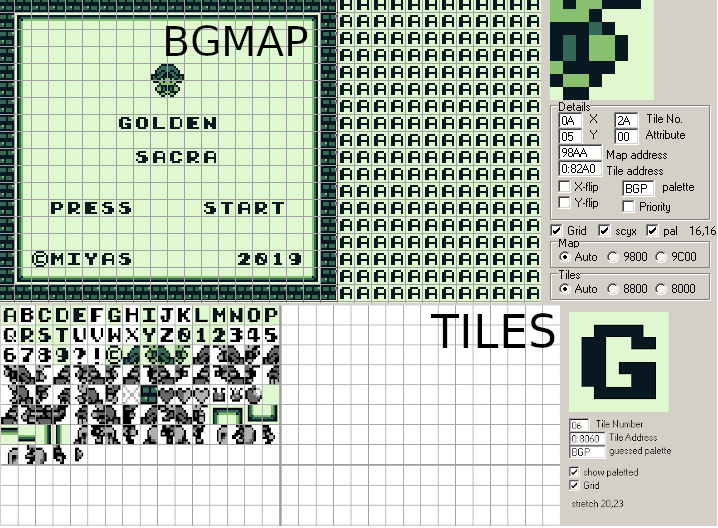
\includegraphics[width=0.7\textwidth]{include/images/VRAM/showbg.png}
\caption{Visualización del VRAM}
\label{figure:bgmap}
\end{figure}

El área que viene a continuación es la \textbf{RAM}. Primero tenemos la sección que pertenece al \textbf{cartucho} (\textbf{\$A000 - \$BFFF}), por lo que puede (o no) que lo tengamos disponible. No es un requisito que los cartuchos tengan este espacio de RAM, pero de hacerlo siempre nos viene bien. Si no estás seguro de disponer de el, mejor no lo uses. Luego está la \textbf{RAM interna} o \textbf{Work RAM} (\textbf{\$C000 - \$DFFF}), donde podremos almacenar los valores que necesitemos mantener a lo largo de los distintos ciclos de cómputo.
\\ \\
El \textbf{espejo de RAM} (\textbf{\$E000 - \$FDFF}) es un espacio de memoria desperdiciado. Es altamente recomendado \textbf{no guardar nada aquí}.
\\ \\
Ahora llegamos a la \textbf{OAM} (\textbf{\$FE00 - \$FE9F}), también conocido como Sprite RAM. Aquí es donde vamos a guardar todos nuestros sprites.
\\ \\
Con el área de \textbf{HRAM} (\textbf{\$FF80 - \$FFFE}) veremos más adelante que se le puede dar buen uso. Y finalmente, el último byte de todos (\textbf{\$FFFF}), es la \textbf{activación de interrupciones}.

\clearpage

\section{Organización de la ROM}

Una pregunta que nos deberíamos hacer siempre es: \textbf{¿dónde debemos programar?} Está claro que nuestro código se va a almacenar en la ROM pero, ¿en cualquier sitio? La respuesta es no, puesto que tiene una organización específica que, si no se respeta, nuestro juego puede que no llegue ni tan siquiera a ejecutar.
\\ \\
Lo mejor es definir en una tabla las distintas posiciones de memoria en los que está compuesta la ROM y que no debemos pasar por alto:

\begin{table}[h!]
\centering
\begin{tabular}{|c|c|c|}
\hline
\multicolumn{3}{|c|}{\textbf{Esquema Memoria ROM}}                                                                          \\ \hline
\textbf{Inicio} & \textbf{Final} & \textbf{Descripción}                                              \\ \hline
00              & 100  & Vectores de interrupción.               \\ \hline
100             & 103  & Entrada a la ejecución del programa.    \\ \hline
104             & 14E  & Cabecera del cartucho.                  \\ \hline
14F             & 3FFF & Lógica del programa.                    \\ \hline
4000            & 7FFF & Segundo banco. Intercambiable.          \\ \hline
\end{tabular}
\caption{Esquema Memoria ROM}
\label{table:4}
\end{table}

El rango \textbf{\$0000-\$0100} son los llamados \textbf{vectores de interrupción}. Según vayamos necesitándolo, veremos que la Game Boy dispone de distintas \textbf{funciones} las cuales pueden ser \textbf{llamadas en cualquier momento del programa}.
\\ \\
La \textbf{cabecera del cartucho} (\textbf{\$0104 - \$014E}) se puede descomponer mucho más, pero lo veremos en profundidad cuando comencemos a programar, por lo que no es necesario explicarlo aquí.

\clearpage

\section{Inputs}
\label{anexo_input}

A la hora de controlar cuándo se han pulsado los botones de la Game Boy tenemos un único registro (\$FF00) que contiene la información de los diferentes 8 botones. Este byte funciona como una especie de matriz:

\begin{figure}[h]
\centering
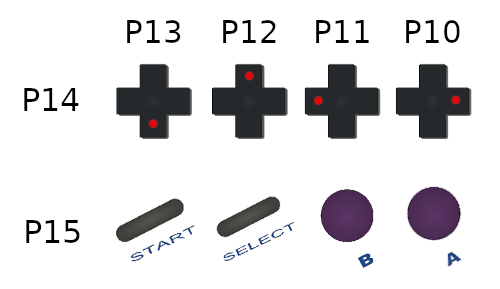
\includegraphics[width=0.5\textwidth]{include/images/GameBoy/PAD.png}
\caption{Distribución del PAD}
\label{figure:pad}
\end{figure}

La nomenclatura P1N que se ha seguido en la imágen no significa otra cosa que ``Player 1'' seguido del número del bit del registro. De esta forma, si quisiésemos guardarnos los valores de los botones A, B, Start o Select pondríamos el bit 5 con valor 1 y el bit 4 con valor 0.
\\ \\
Hay que tener en cuenta que los valores que nos devuelve este registro están al revés de como solemos pensar. Con esta afirmación me refiero a que si un botón está pulsado, el valor que aparecerá es 0 y no 1. No es un problema muy serio a tener en cuenta ya que podemos hacer un complementario para tener los valores de la forma habitual (1 = si, 0 = no). 

\section{Interrupciones}
\label{anexo:interruptions}
Las interrupciones, como su nombre indica, son \textbf{procesos por lo que la CPU deja en pausa la ejecución} de la lógica del juego para saltar a una posición de memoria determinada, también llamada vector. Son útiles ya que, entre otros, se pueden dar en cualquier parte de nuestro código.
\\ \\
La mayoría de las CPU's tienen un ``\textbf{master flag}'' para las interrupciones. La Z80 que lleva la Game Boy no es distinta, pero hay registros adicionales específicos de la consola. El registro maestro es el \textbf{IME} (\textbf{Interrupt Master Enable}) el cual es \textbf{desactivado con el opcode DI}, con lo que no se daría ninguna interrupción. Por el contrario, \textbf{se activa con EI}, \textbf{produciéndose todas las interrupciones} que nosotros especifiquemos \textbf{en el registro IE} (\textbf{Interrupt Enable, \$FFFF}). De manera complementaria, tenemos el \textbf{registro IF} (\textbf{Interrupt Flag, \$FF0F}), el cual indica qué interrupción se ha activado.

\clearpage

El \textbf{proceso} que se da cada vez que se da una interrupción es el siguiente:

\begin{enumerate}
	\item Cuando una interrupción se produce, su bit del registro IF se pone a 1.
	\item Si el IME y el bit representativo de la interrupción en el registro IE están activos, se producen los siguientes tres pasos.
	\item El registro IME se desactiva para prevenir otra interrupción mientras se procesa ya una.
	\item El registro PC (Program Counter) se pushea al stack.
	\item Se hace un salto al vector de la interrupción.
\end{enumerate}


Hay \textbf{5 tipos} de interrupciones:

\begin{table}[h!]

\centering
\begin{tabular}{|c|l|l|l|c|}

\hline

\multicolumn{4}{|c|}{\textbf{Interrupción}}         & \textbf{Dirección de memoria} \\ \hline

\multicolumn{4}{|c|}{Vertical Blank}       & 0040                 \\ \hline

\multicolumn{4}{|c|}{Estado del LCD}       & 0048                 \\ \hline

\multicolumn{4}{|c|}{Temporizador}         & 0050                 \\ \hline

\multicolumn{4}{|c|}{Serial Link}          & 0058                 \\ \hline

\multicolumn{4}{|c|}{Pulsación del Joypad} & 0060                 \\ \hline

\end{tabular}

\caption{Interrupciones de la Game Boy}
\label{table:interrupts}
\end{table}

\begin{itemize}
	\item \textbf{V-Blank:} Se produce alrededor de 60 veces por segundo. Ocurre cuando se redibuja la última línea de la pantalla, que es cuando el hardware no esta haciendo uso de la memoria de vídeo. Dura alrededor de 1'1ms.
    \item \textbf{Estado del LCD:} Hay varias razones por las que esta interrupcion se puede dar, descritas en el registro STAT (\$FF40).
    \item \textbf{Temporizador:} Se produce cuando el registro TIMA (\$FF05) cambia su valor de \$FF a \$00.
    \item \textbf{Serial Link:} Se produce cuando una trasferencia de datos se ha completado a través del puerto del cable link.
    \item \textbf{Pulsación del Joypad:} Se produce cuando el usuario presiona cualquier botón. Debido al efecto ``\textit{bouncing}''\footnote{El ``\textit{bouncing}'' es aquel efecto que, a nivel microscópico, cuando se pulsa un botón, los contactos rebotan. Esto genera pequeños saltos de señal que el hardware lee.}, la parte del software debería tener presente que esta interrupción puede producirse varias veces de forma consecutiva.
\end{itemize}

\clearpage

\section{GPU}
\label{anexo_gpu}

La \textbf{GPU} (\textbf{Graphics Processing Unit}), tambien referenciada en la Game Boy como \textbf{PPU} (\textbf{Picture Processing Unit}), es uno de los principales componentes junto a la CPU. Es la principal vía para mostrar gráficos por pantalla, y gran parte del trabajo del procesador se basa en generarlos para pasárselos a esta. 
\\ \\
Tiene las siguientes \textbf{especificaciones}:

\begin{itemize}
	\item \textbf{2 fondos de pantalla}, una principal y otra secundaria utilizada de ventana.
	\item \textbf{40 sprites}, máximo 10 por línea.
	\item Tiles de tamaño 8x8.
	\item \textbf{4 modos} de dibujado.
	\item 456 ciclos por línea, 70224 por frame.
	\item \textbf{4 colores} en tonos de gris (2-bit).
	\item LCD de 160x144 píxeles (20x18 tiles).
\end{itemize}

Los \textbf{4 modos de dibujado} son los siguientes:

\begin{itemize}
	\item \textbf{Modo 0 - \$00:} H-Blank.
	\item \textbf{Modo 1 - \$01:} V-Blank.
	\item \textbf{Modo 2 - \$10:} Escaneo de OAM.
	\item \textbf{Modo 3 - \$11:} H-Draw. Tiempo en el que se transfieren datos al driver del LCD.
\end{itemize}
\label{d_modes}

Los modos 0, 2 y 3 no ocurren durante el V-Blank, solo durante el V-Draw. En la siguiente imágen puedes ver cuando se da cada una, a excepción del H-Draw que se da siempre que se dibuje un pixel por pantalla:

\begin{figure}[h]
\centering
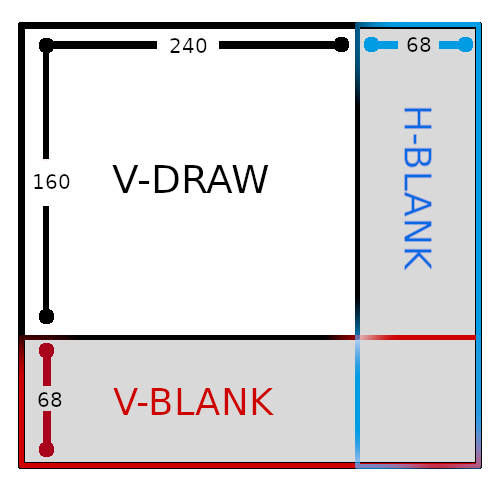
\includegraphics[width=0.3\textwidth]{include/images/VRAM/draw_modes.png}
\caption{Modos de dibujado de la GPU}
\label{figure:draw_modes}
\end{figure}

\clearpage

\subsection{LCD control}

El LCD control se encuentra en la dirección de memoria \$FF40, y es el encargado de controlar todo lo que se dibuja por pantalla. Sus bits tienen los siguientes usos:

\begin{itemize}
	\item \textbf{Bit 7:} Apaga o enciende el LCD. 
	\item \textbf{Bit 6:} Selección de la posición del fondo de pantalla secundaria (0 = \$9800-\$9BFF, 1 = \$9C00-\$9FFF).
	\item \textbf{Bit 5:} Dibuja o esconde la pantalla secundaria.
	\item \textbf{Bit 4:} Selecciona la posición de los tiles que componen las 2 pantallas (0 = \$8800-\$97FF, 1 = \$8000-\$8FFF).
	\item \textbf{Bit 3:} Selecciona la posición de la pantalla principal (0 = \$9800 - \$9BFF, 1 = \$9C00 - \$9FFF).
	\item \textbf{Bit 2:} Tamaño de los sprites (0 = 8x8, 1 = 8x16). En caso de activarlo, cada sprite usará su tile asignado más el siguiente en memoria.
	\item \textbf{Bit 1:} Dibuja o no los sprites (0 = no, 1 = sí).
	\item \textbf{Bit 0:} Dibuja o no los dos fondos de pantalla (0 = no, 1 = sí).
\end{itemize}

\subsection{LCD STAT}

Como hemos comentado previamente, el STAT es el registro que nos muestra en todo momento el estado del LCD. 
\\ \\
Sus bits funcionan de la siguiente manera:

\begin{itemize}
	\item \textbf{Bit 7:} Sin uso.
	\item \textbf{Bit 6:} Interrupción cuando LYC = LY\footnote{LY es la línea por la que el scanline está dibujando y LYC es la seleccionada por el usuario.}.
	\item \textbf{Bit 5:} Modo 10 (OAM Scan).
	\item \textbf{Bit 4:} Modo 01 (V-Blank).
	\item \textbf{Bit 3:} Modo 00 (H-Blank).
	\item \textbf{Bit 2:} Flag de coincidencia. Se activa si LYC = LY.
	\item \textbf{Bit 0-1:} Modo de dibujado del LCD (Ver apartado~\ref{d_modes}).
\end{itemize}

Los bits que van del 3 al 6 selecciona las condiciones por la que la interrupción STAT pueda ser dada. Seleccionar más de una de manera simultánea puede generar un bloqueo.

\subsection{LCD Color Display (Solamente CGB)}
\label{anexo:lcd_color}

En caso de utilizar una GBC, la pantalla LCD puede llegar a mostrar un total de 32 tonos en cada canal de color RGB, dando como resultado un total de 32768 colores diferentes. Las paletas constan solamente de 4 colores, escogidos del total ya mencionado.
\\ \\
Igual que ocurre con el modo DMG, podemos utilizar paletas independientes para el BG y el OBJ. Sin embargo, como el canal OBJ dispone de un canal transparente, este solamente tendrá 3 colores en total.

\subsubsection{LCD Palettes}

Cada paleta del modo CGB son representadas mediante 2 bytes, en los cuales cada canal de color RGB viene a su vez representado por 5 bits. El bit más alto queda en desuso.

Los datos se escriben mediante los registros de especificación y los registros de escritura. Los 6 bits del registro de especificación, como su nombre indica, precisa la dirección de escritura en la que van a acabar guardados los datos que sean introducidos en el registro de escritura. Si el bit más alto del registro de especificación se pone a 1, el registro de escritura se incrementará de forma automática (la dirección a incrementar es la especificada en los 6 bits bajos).
\\ \\
Los registros de especificación a utilizar para las paletas de color en modo CGB son \$FF68 y \$FF6A, y los registros de escritura \$FF69 y \$FF6B, siendo utilizadas para las paletas de BG y OBJ respectivamente.

\begin{figure}[h]
\centering
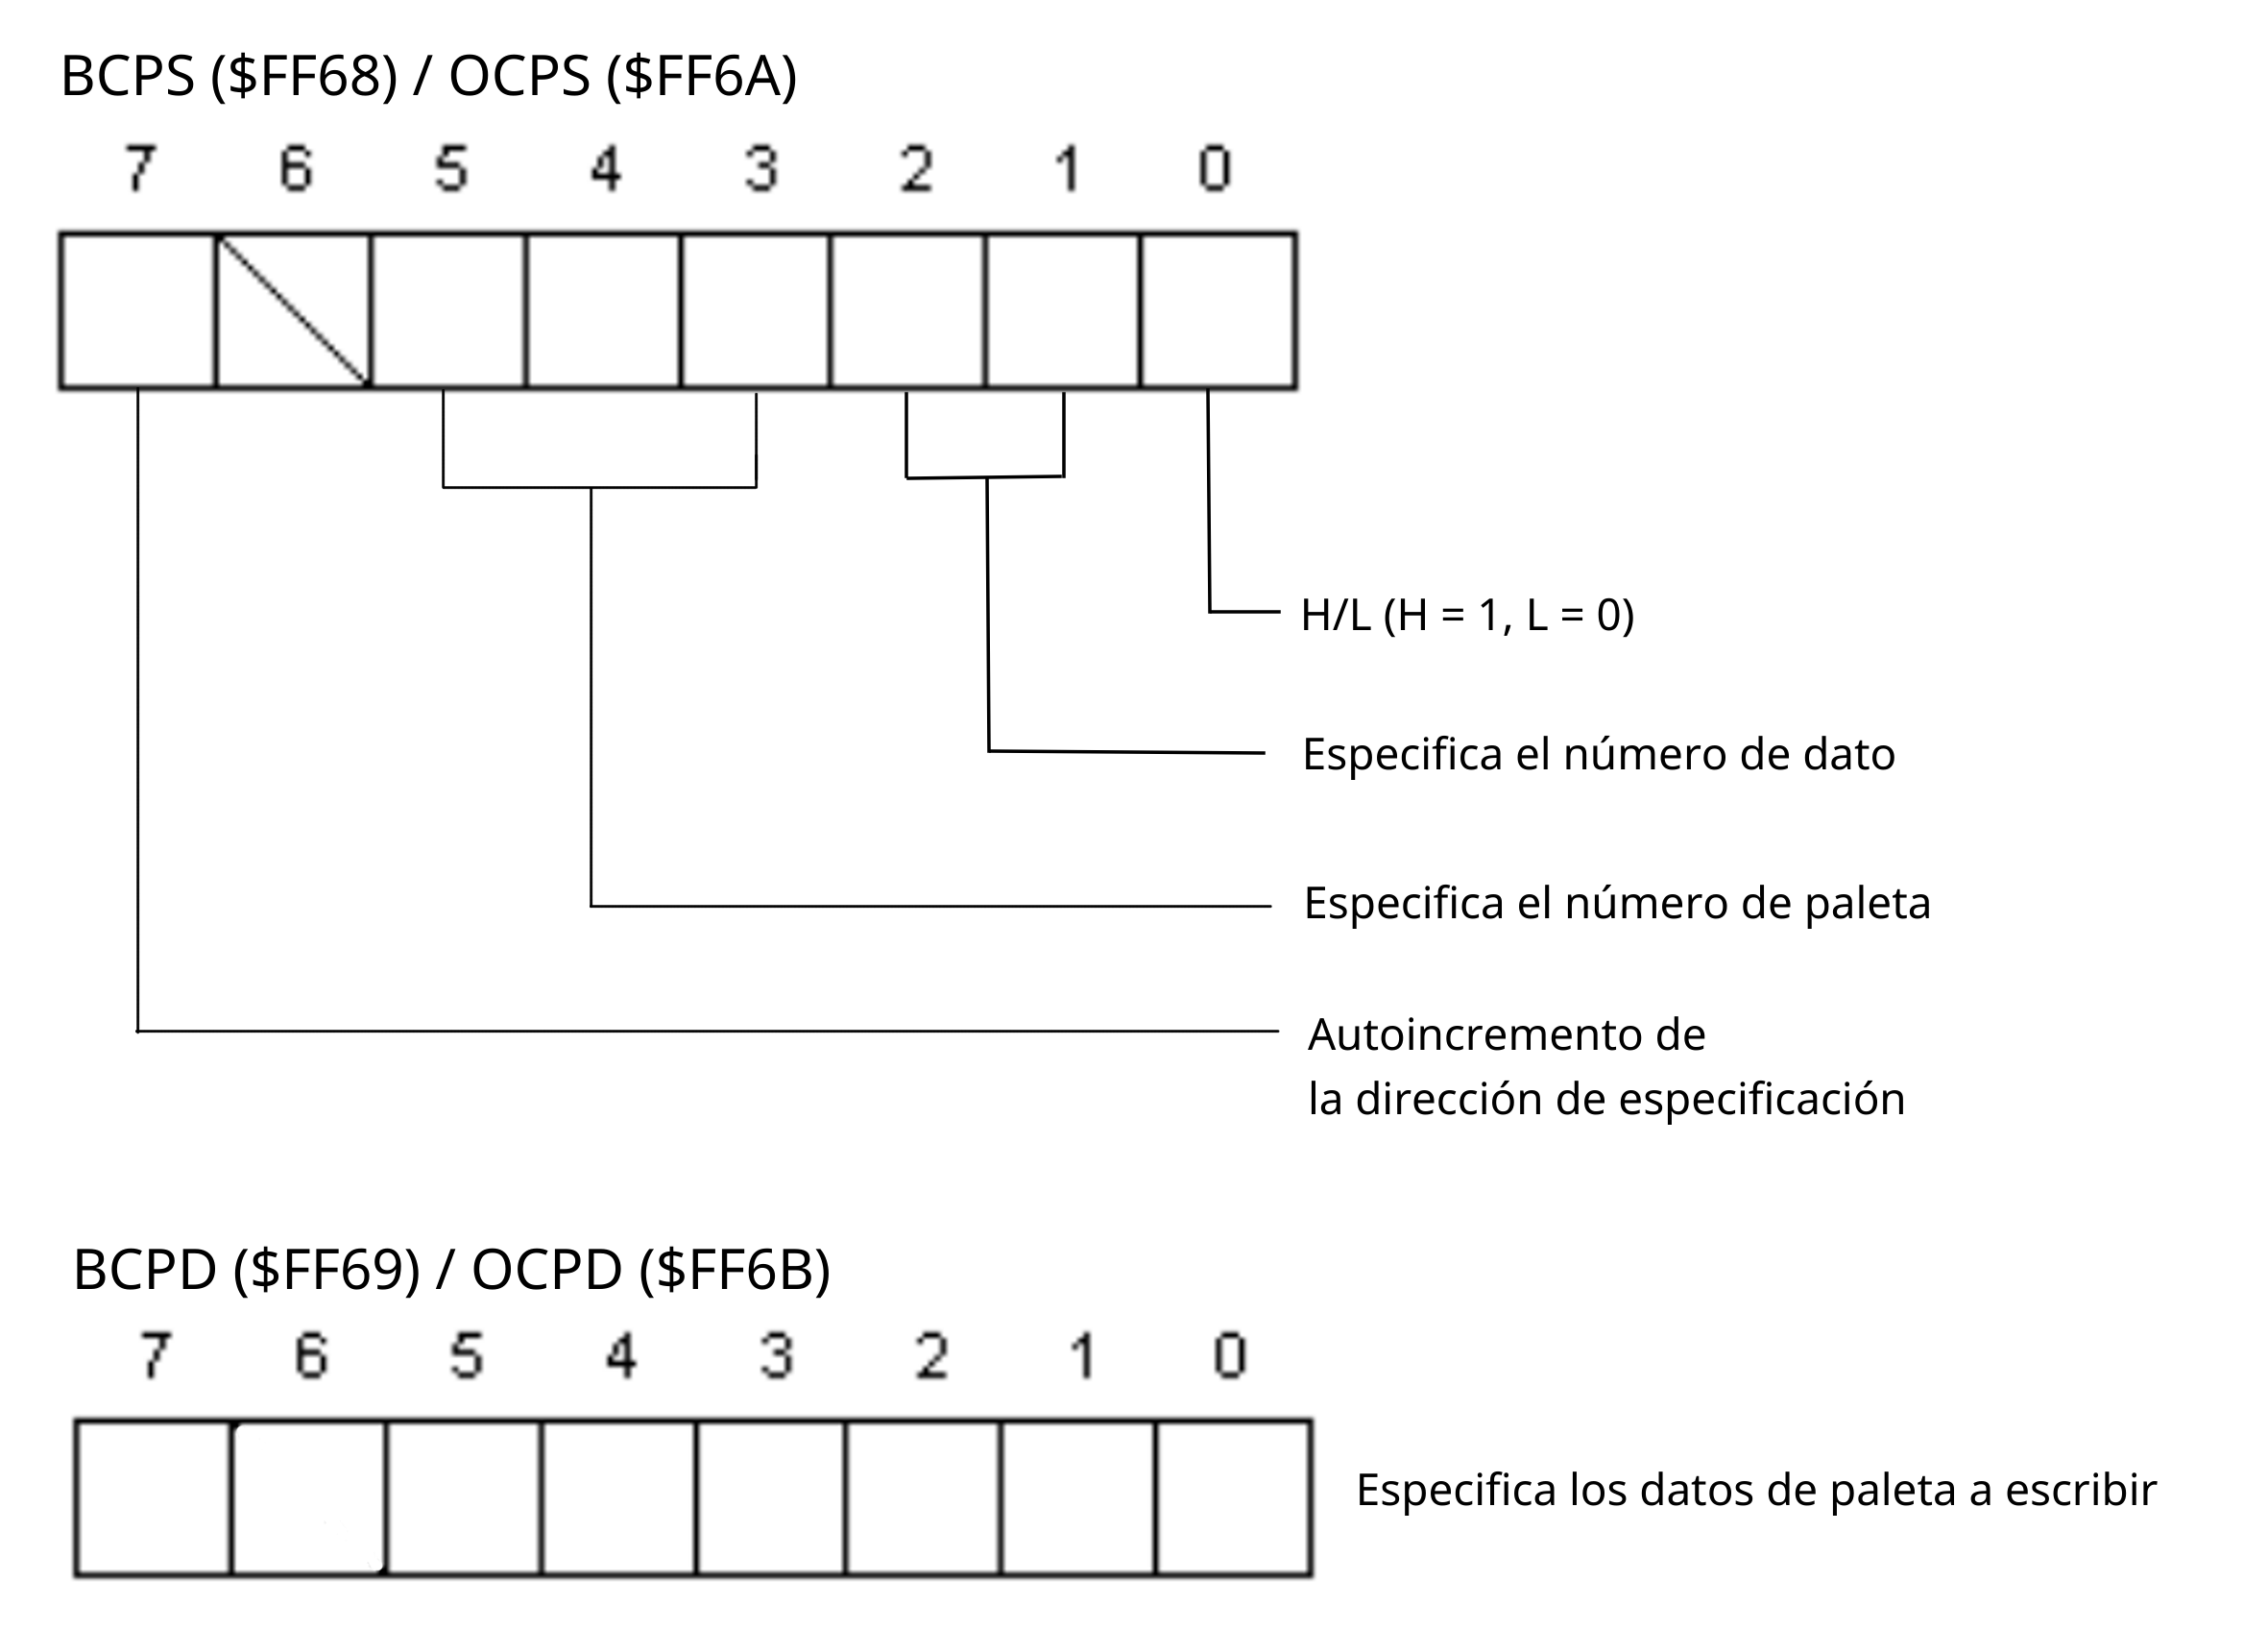
\includegraphics[width=0.8\textwidth]{include/images/GameBoy/registrospaleta.png}
\caption{Representación Gráfica de los Registros de Especificación y Escritura en Modo CGB}
\label{figure:PalRegisters}
\end{figure}

\clearpage

\section{Sonido}
\label{anexo:sonido}

La Game Boy dispone de 4 canales diferentes, los cuales son programables e independientes los unos de los otros:

\begin{itemize}
	\item \textbf{Canal 1:} Tono\footnote{El tono o altura del sonido es el atributo que nos hace percibir los sonidos más agudos o graves.} y portamento\footnote{El portamento es la transición entre sonidos graves y agudos para impedir percibir una discontinuidad.}. Se trata de una onda cuadrada a la que le podemos modificar el régimen de trabajo.
	
	\item \textbf{Canal 2:} Tono. Al igual que el Canal 1, es una onda cuadrada de régimen de trabajo modificable.
	
	\item \textbf{Canal 3:} Onda programable. Tiene una RAM de onda de 32 valores (4 bits). No dispone de envolvente de amplitud, a diferencia de los otros 3 canales.
	
	\item \textbf{Canal 4:} Ruido blanco.
	
\end{itemize}

Vamos a explicar varios conceptos teóricos de manera que podamos entenderlas sin necesidad de consultar otros documentos:
\\ \\
El régimen de trabajo o ciclo útil se refiere al porcentaje de tiempo que dura el nivel alto respecto al nivel bajo de una onda cuadrada.

\begin{figure}[h]
\centering
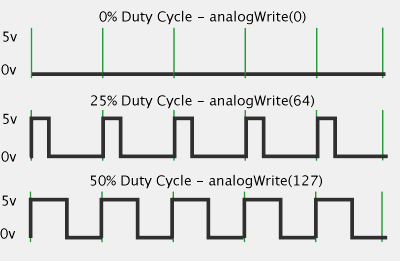
\includegraphics[width=0.5\textwidth]{include/images/manual/cycle.png}
\caption{Ejemplo Gráfico de Ciclo Útil de una Onda}
\label{figure:cycle}
\end{figure}

Por otro lado, la envolvente de amplitud es un gráfico en el que se muestra la evolución a lo largo del tiempo del ya nombrado atributo correspondiente a una onda. Esto es, desde el momento de su emisión, hasta su desaparición.
\\ \\
Esta envolvente nos da la información de si el tiempo de ataque es abrupto, cuánto tiempo se mantiene el sonido, y si su extinción se va produciendo poco a poco o de manera inmediata.

\begin{figure}[h]
\centering
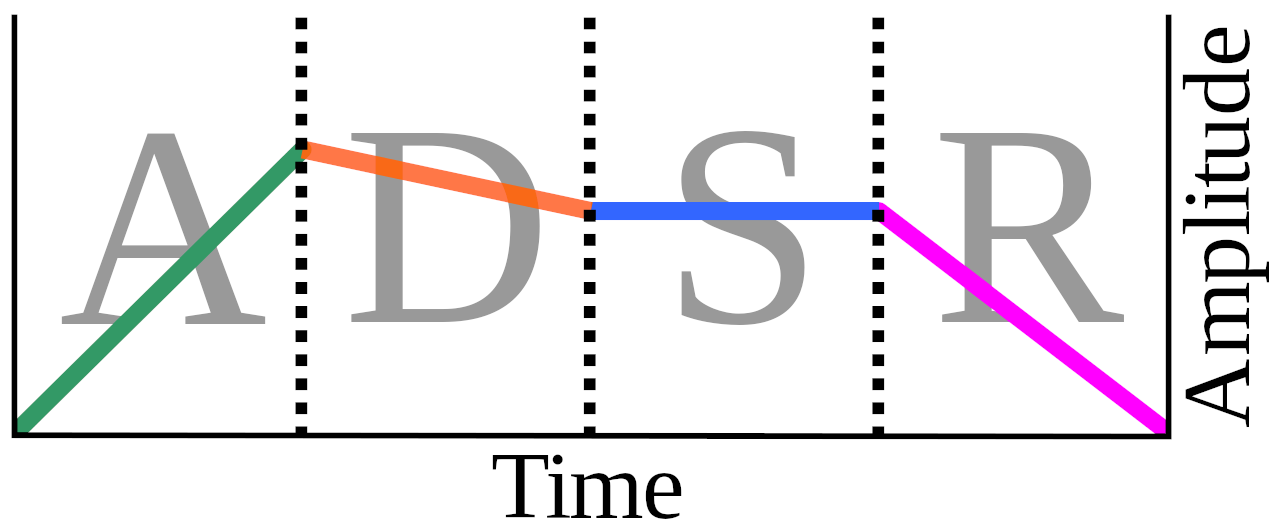
\includegraphics[width=0.5\textwidth]{include/images/manual/envelope.png}
\caption{Ejemplo Gráfico de Envolvente de Amplitud}
\label{figure:envelope}
\end{figure}

A continuación vamos a ver, como no, los registros que nos van a hacer falta del sistema de sonido:

\subsection{Canal 1 - Tono \& Portamento}
	
	\begin{itemize}
		\item \textbf{\$FF10:} Registro de portamento.
	
		Los bits del 6 al 4 especifican la duración del portamento. El bit 3 indica el incremento/decremento.	Los bits del 2 al 0 indican, por último, el desplazamiento.
		
		\begin{table}[h!]
			\centering
			\begin{tabular}{|c|l|l|l|c|}
				\hline
				\multicolumn{4}{|c|}{000}       & Apagado                 				\\ \hline
				\multicolumn{4}{|c|}{001}       & 7.8 ms  (1/128Hz)                 				\\ \hline
				\multicolumn{4}{|c|}{010}       & 15.6 ms (2/128Hz) 					\\ \hline
				\multicolumn{4}{|c|}{011}       & 23.4 ms (3/128Hz) 					\\ \hline
				\multicolumn{4}{|c|}{100} 		& 31.3 ms (4/128Hz)              				\\ \hline
				\multicolumn{4}{|c|}{101} 		& 39.1 ms (5/128Hz) 					\\ \hline
				\multicolumn{4}{|c|}{110} 		& 46.9 ms (6/128Hz) 					\\ \hline
				\multicolumn{4}{|c|}{111} 		& 54.7 ms (7/128Hz) 					\\ \hline
			\end{tabular}
			\caption{Duraciones del Portamento}
			\label{table:portamento}
		\end{table}
		
		\item \textbf{\$FF11:} Duración del ciclo de trabajo.
	
		Los bits 7 y 6 se utilizan para indicar el ciclo de trabajo. Los bits restantes sirven para especificar la longitud de onda.
		
		\begin{table}[h!]
			\centering
			\begin{tabular}{|c|l|l|l|c|}
				\hline
				\multicolumn{4}{|c|}{00}       & 12.5\% 								\\ \hline
				\multicolumn{4}{|c|}{01}       & 25\% 									\\ \hline
				\multicolumn{4}{|c|}{10}       & 50\% 									\\ \hline
				\multicolumn{4}{|c|}{11}       & 75\%
				\\ \hline
			\end{tabular}
			\caption{Ciclos de trabajo}
			\label{table:cycle}
		\end{table} 	
		
		\item \textbf{\$FF12:} Envolvente de amplitud.
		
		Los bits del 7 al 4 indican el volumen inicial (desde \$00 hasta \$0F). El bit 3, la dirección de la envolvente. Los bits 2-0 son el periodo.	
		
		\item \textbf{\$FF13:} Frecuencia baja.

		Los 8 bits nos especifican la frecuencia baja. En total son 11 bits, pero los 3 restantes están en la dirección de memoria \$FF14.		
		
		\item \textbf{\$FF14:} Frecuencia alta.
		
		El bit 7 es el iniciador (cuando se le da valor 1, el sonido se reinicia). El bit 6 activa o desactiva la longitud. Este bit es el único que se puede leer, el resto son de escritura. Los bits 2-0 son los correspondientes a la frecuencia baja.		
		
	\end{itemize}

\subsection{Canal 2 - Tono}
	
	\begin{itemize}
		\item \textbf{\$FF16:} Duración del ciclo de trabajo.
		
		Los bits 7 y 6 se utilizan para indicar el ciclo de trabajo. Los bits restantes sirven para especificar la longitud de onda. Los valores correspondientes son los mismos a la de la tabla \textbf{\hyperref[table:cycle]{9.6}}.
		
		\item \textbf{\$FF17:} Envolvente de amplitud.
	
		Los bits del 7 al 4 indican el volumen inicial (desde \$00 hasta \$0F). El bit 3, la dirección de la envolvente. Los bits 2-0 son el periodo.			
		
		\item \textbf{\$FF18:} Frecuencia baja.
		
		Los 8 bits nos especifican la frecuencia baja. En total son 11 bits, pero los 3 restantes están en la dirección de memoria \$FF14.		
		
		\item \textbf{\$FF19:} Frecuencia alta.
		
		El bit 7 es el iniciador (cuando se le da valor 1, el sonido se reinicia). El bit 6 activa o desactiva la longitud. Este bit es el único que se puede leer, el resto son de escritura. Los bits 2-0 son los correspondientes a la frecuencia baja.		
		
	\end{itemize}
	
\subsection{Canal 3 - Onda Programable}
	
	\begin{itemize}
		\item \textbf{\$FF1A:} Encendido/Apagado.
		
		El valor del bit 7 nos indica si el sonido está encendido o apagado.		
		
		\item \textbf{\$FF1B:} Longitud.
		
		Los 8 bits especifican la longitud de onda. Solamente se utiliza si el bit 6 de \$FF1E esta a 1.		
		
		\item \textbf{\$FF1C:} Nivel de volumen.
		
		Los bits 6 y 5 indican el nivel de salida.
		
		\begin{table}[h!]
			\centering
			\begin{tabular}{|c|l|l|l|c|}
				\hline
				\multicolumn{4}{|c|}{00}       & Apagado								\\ \hline
				\multicolumn{4}{|c|}{01}       & 100\% 									\\ \hline
				\multicolumn{4}{|c|}{10}       & 50\% 									\\ \hline
				\multicolumn{4}{|c|}{11}       & 25\%
				\\ \hline
			\end{tabular}
			\caption{Niveles de volumen}
			\label{table:vol}
		\end{table} 
		
		\item \textbf{\$FF1D:} Frecuencia baja.
		
		Los 8 bits nos especifican la frecuencia baja. En total son 11 bits, pero los 3 restantes están en la dirección de memoria \$FF14.		
		
		\item \textbf{\$FF1E:} Frecuencia alta.
	
		El bit 7 es el iniciador (cuando se le da valor 1, el sonido se reinicia). El bit 6 activa o desactiva la longitud. Este bit es el único que se puede leer, el resto son de escritura. Los bits 2-0 son los correspondientes a la frecuencia baja.		
		
		\item \textbf{\$FF30:} Patrón de onda.
		
		Almacena la forma de la onda para generar datos de sonido aleatorios. Contiene 32 muestras de 4 bits que se reproducen con los 4 bits altos en primer lugar.		
		
	\end{itemize}
	
\subsection{Canal 4 - Ruido Blanco}

	El ruido blanco surge variando de manera aleatoria la amplitud de una frecuencia.
	
	\begin{itemize}
		\item \textbf{\$FF20:} Longitud.
		
		Los 8 bits especifican la longitud de onda. Solamente se utiliza si el bit 6 de \$FF1E esta a 1.		
		
		\item \textbf{\$FF21:} Envolvente de amplitud.
		
		Los bits del 7 al 4 indican el volumen inicial (desde \$00 hasta \$0F). El bit 3, la dirección de la envolvente. Los bits 2-0 son el periodo.			
		
		\item \textbf{\$FF22:} Contador polinómico.
		
		Los bits del 7 al 4 sirven para especificar la frecuencia de reloj con la que la amplitud va a cambiar de forma aleatoria. El bit 3 especifica la medida del contador. Los bits restantes (2-0) hacen referencia al radio de división de las frecuencias.
		
		\item \textbf{\$FF23:} Disparador o Iniciador.
		
		El bit 7 es el iniciador (cuando se le da valor 1, el sonido se reinicia). El bit 6 activa o desactiva la longitud.
		
	\end{itemize}
	
\subsection{Registros de Uso General}
	
	\begin{itemize}
		\item \textbf{\$FF24:} Control de volumen.
		
		Controla tanto el volumen de los canales izquierdos como los derechos.		
		
		\item \textbf{\$FF25:} Selección de salida de canal.
		
		Indica si un canal debe salir por la izquierda o por la derecha. Las terminales de salida se nombran como SO1 y SO2.
		
		\begin{table}[h!]
			\centering
			\begin{tabular}{|c|l|l|l|c|}
				\hline
				\multicolumn{4}{|c|}{Bit 7}       & Canal 4 - SO2							\\ \hline
				\multicolumn{4}{|c|}{Bit 6}       & Canal 3 - SO2								\\ \hline
				\multicolumn{4}{|c|}{Bit 5}       & Canal 2 - SO2 									\\ \hline
				\multicolumn{4}{|c|}{Bit 4}       & Canal 1 - SO2
				\\ \hline
				\multicolumn{4}{|c|}{Bit 3}       & Canal 4 - SO1
				\\ \hline
				\multicolumn{4}{|c|}{Bit 2}       & Canal 3 - SO1
				\\ \hline
				\multicolumn{4}{|c|}{Bit 1}       & Canal 2 - SO1
				\\ \hline
				\multicolumn{4}{|c|}{Bit 0}       & Canal 1 - SO1
				\\ \hline
			\end{tabular}
			\caption{Niveles de volumen}
			\label{table:vol}
		\end{table} 
		
		\item \textbf{\$FF26:} Apagado o encendido del sonido.
		
		El bit 7 en el controlador general (apaga o enciende todos los canales). El bit 3 controla el canal 4, el bit 2 el canal 3, etc. Desactivar el sonido puede ahorrar hasta un 16\% de batería.		
		
	\end{itemize}

\cleardoublepage %salta a nueva página impar

\chapter{Conclusiones Finales}

En esta sección voy a hacer unas breves conclusiones respecto al resultado definitivo del proyecto y todo lo que se ha aprendido a lo largo de su desarrollo.

\section{Estado del Producto}

Existen muchas funcionalidades definidas en el \textbf{Game Design Document} que no se han llegado a finalizar, como el poder subir de nivel al ganar experiencia, el poder interactuar con distintos NPC's, o que existan distintas mazmorras con un jefe final en cada una de ellas. Podemos decir entonces que el juego, en el estado que se encuentra actualmente, es muy mejorable. 
\\ \\
Sin embargo, es un \textbf{proyecto cerrado, divertido y con sentido}, el cual cumple con su cometido perfectamente. Por ende, es un proyecto que en el futuro se puede enseñar en un portfolio con mucho orgullo.
\\ \\
Por otro lado, como es normal, a lo largo del desarrollo han surgido \textbf{nuevas ideas} que pueden mejorar mucho la experiencia de usuario. Aún así, lo propio fue centrarse en las tareas marcadas como principales desde principio de desarrollo y, en caso de dar tiempo, hacerlas. Se van a nombrar en el siguiente apartado.

\section{Posibles Futuras Mejoras}

Como hemos comentado, Golden Sacra dispone de un amplio abanico de posibles mejoras para mejorar la experiencia de juego:

\begin{itemize}
		\item \textbf{Generación Procedimental:} Esto nos puede servir para tener un número indefinido de pisos y mazmorras. Al disponer de una consola muy limitada en cuanto a memoria, hacer un algoritmo de semilla (por ejemplo) para generar todos los pisos que compongan una mazmorra, nos puede ahorrar tanto en espacio como en tiempo. Además, esto conseguiría que los pisos se volviesen a generar cada vez que el jugador entre a la misma mazmorra, obteniendo un resultado diferente y, por tanto, aumentando de este modo la rejugabilidad.
		
		\item \textbf{Animaciones:} Si bien en el producto se han conseguido introducir todas las animaciones básicas, faltan muchas que aumentan la satisfacción general del usuario, como las de morir o consumir un objeto.
		
		\item \textbf{Mejorar la Inteligencia Artificial:} Como se ha explicado a lo largo del desarrollo, el comportamiento de los enemigos no se pueden considerar como una "inteligencia artificial". Habría que definirlos más bien como patrones. Posibles mejoras son la de que un enemigo, al ver al jugador en un radio, decida cerrar una puerta para que este tenga que proceder por otro camino algo más largo. Detalles como este que acabo de describir pueden dotar al proyecto de una mayor variedad a la hora de tomar decisiones.
		
		\item \textbf{Más Niveles:} Actualmente solo disponemos de una mazmorra con 3 pisos. Una de las mejoras más claras es la de expandir este número de niveles disponibles, los cuales se vayan desbloqueando según el jugador avance y consiga llegar al último piso de una mazmorra específica.
	
	\item \textbf{Nuevos Objetos:} Disponer solamente de 3 objetos está bien desde el punto de vista a corto plazo. Si queremos hacer un proyecto entretenido en todas las horas de juego que este pueda ofrecer, necesitamos disponer de una amplia gama de objetos que puedan decantar la balanza entre morir o salvarse.
	\end{itemize}

\section{Opiniones Personales}

Creo que como ingeniero he conseguido avanzar y mejorar bastante a lo largo del desarrollo. El lenguaje ensamblador no solo te hace entender mejor el funcionamiento de la máquina objetivo (una Game Boy en este caso), sino que además te ayuda a entender mejor lo que está ocurriendo por debajo a la hora de programar en cualquier otro lenguaje de alto nivel.
\\ \\
Cuando entré en la carrera siempre tuve la incógnita de cómo se podría llegar a hacer un juego para esta consola, y a parte de poder decir "ya se hacerlo", puedo decir también "ya lo he hecho".
\\ \\
Comenzar proyectos nuevos siempre da miedo, y más cuando los debes hacer por tu cuenta, sin nadie que te pare los pies ante las posibles malas decisiones, ni que te pueda ayudar ante los problemas que se te pongan de frente. Sin embargo, al igual de que el riesgo es mayor, la recompensa también lo es. Mis conocimientos han aumentado en gran medida, y esto se puede comprobar con el simple hecho de que volvería a hacer todo desde 0. Y aún así espero que, en caso de hacerlo, una vez termine pueda volver a decir exactamente lo mismo.

